\subsection{Concetto generale di Sistema. I sistemi che ci interessano includono HW SW e aspetti organizzativi (persone, processi).}
\begin{itemize}
    \item Una raccolta mirata di componenti interconnessi che lavorano insieme verso un obiettivo comune. Un sistema può includere software, hardware meccanico, elettrico ed elettronico ed essere gestito da persone. I componenti di sistema dipendono da altri componenti di sistema. Le proprietà e il comportamento dei componenti del sistema sono indissolubilmente mescolati
\end{itemize}
\subsection{Problematiche dell’ingegneria dei sistemi e relazioni con l’IS.}
\begin{itemize}
    \item I sistemi di grandi dimensioni sono generalmente progettati per risolvere problemi "malvagi"
    \item L'ingegneria dei sistemi richiede un grande coordinamento in tutte le discipline
    \begin{itemize}
        \item Quasi infinite possibilità di compromessi di progettazione tra i componenti
        \item Diffidenza reciproca e mancanza di comprensione tra le discipline ingegneristiche
    \end{itemize}
    \item I sistemi devono essere progettati per durare molti anni in un ambiente che cambia
    \item La percentuale di software nei sistemi è in aumento. L'elettronica per uso generale basata su software sta sostituendo i sistemi per uso speciale
    \item I problemi di ingegneria dei sistemi sono simili ai problemi di ingegneria del software
    \item Il software è (purtroppo) visto come un problema nell'ingegneria dei sistemi. Molti grandi progetti di sistema sono stati ritardati a causa di problemi del software
    \item Spesso viene richiesto al software di "compensare" la "rigidità" dell'hardware!
    \item E’ quindi necessario inquadrare l’attività di sviluppo del SW nel ambito più vasto e generale del processo di ingegnerizzazione del Sistema in cui il SW sarà inserito.
    \item Bisogna quindi considerare lo scopo del Sistema, i requisiti (di business) cui va incontro, i ruoli delle varie componenti (varie tipologie di dispositivi HW, le persone e i processi coinvolti, alter procedure a DB coinvolti, …)
    \item Concentrarsi solo e immediatamente sul SW senza avere una visione più generale ‘di Sistema’ non è corretto!
\end{itemize}
\subsection{Proprietà emergenti. P. funzionale e p. non funzionali. Shall-not properties.}
\begin{itemize}
    \item Proprietà emergenti: sono proprietà del sistema visto come tutt'uno piuttosto che proprietà dei singoli componenti e sono conseguenze delle relazioni tra i componenti del sistema (possono essere misurate solo dopo l'integrazione dei vari componenti nel sistema). Es. peso, usabilità e affidabilità.
    \item Proprietà (emergenti) funzionali: riguardano \textbf{come un sistema funziona}, i.e. la relazione input/ouput. Es. una bicicletta ha la proprietà funzionale di essere un dispositivo di trasporto una volta assemblata dai suoi componenti.
    \item Proprietà (emergenti) non funzionali: riguardano il \textbf{comportamento del sistema} nel suo ambiente operativo. Es. affidabilità, prestazioni, sicurezza, usabilità e protezione.
    \item \textit{shall-not properties}: sono proprietà che il sistema \textbf{non dovrebbe esibire}.
\end{itemize}
\subsection{Cambiamento dei fattori umani/organizzativi e loro importanza.}
\begin{itemize}
    \item Process changes: Il sistema richiede modifiche ai processi di lavoro nell'ambiente?
    \item Job changes: Il sistema diminuisce le abilità degli utenti in un ambiente o fa cambiare il loro modo di lavorare?
    \item Organisational changes: Il sistema cambia la struttura del potere politico in un'organizzazione?
\end{itemize}
\subsection{Processo di systems engineering e fasi principali.}
\begin{itemize}
    \item in genere si usa il modello \textit{waterfall} che consiste nella definizione dei requisiti, nel design del sistema, nello sviluppo dei sottosistemi, nell'integrazione, poi l'installazione, l'evoluzione e infine la de-commissione.
\end{itemize}
\subsection{Problemi nel System requirements}
\begin{itemize}
     \item Modifica in base al sistema specificato
     \item È necessario anticipare gli sviluppi hardware/comunicazioni per tutta la durata del sistema
     \item Difficile definire requisiti non funzionali (in particolare) senza un'impressione della struttura dei componenti del sistema.
\end{itemize}
\subsection{Problemi nel System design}
\begin{itemize}
     \item I requisiti di partizionamento su hardware, software e componenti umani possono comportare molte negoziazioni
     \item Spesso si presume che i problemi di progettazione difficili vengano risolti prontamente utilizzando il software
     \item Le piattaforme hardware potrebbero non essere appropriate per i requisiti software, quindi il software deve compensare questo
\end{itemize}
\subsection{Evoluzione e legacy}
\begin{itemize}
    \item I grandi sistemi hanno grandi periodi di vita, devono evolvere per rispettare i requisiti in cambiamento.
    \item Sistemi legacy: sistemi ancora in uso che sono stati sviluppati nel passato con tecnologie, metodologie, procedure, lavorazioni \dots che sono nel frattempo diventate obsolete, ciò li rende di difficile cambiamento perché la modifica di un componente comporta la modifica di altri componenti.
\end{itemize}
\subsection{System Procurement: due possibilità, modello dei processi}
\begin{itemize}
    \item sviluppo del sistema da parti pre-confenzionate (COTS -- components off the shelf)
    \item sviluppo del sistemi da zero (esempio hardware: si scelgono i vari componenti: cpu, bluetooth, memoria, porte \dots e vengono montate su una board)
\end{itemize}
\subsection{Modello Contractor/subcontractor}
\begin{itemize}
    \item La fornitura di grandi sistemi hardware/software si basa generalmente su alcuni principali contraenti
    \item I sotto-contratti vengono stipulati con altri fornitori per alcune parti del sistema
    \item Il cliente è in contatto con il contraente principale e non tratta direttamente con i sotto-contraenti
    
    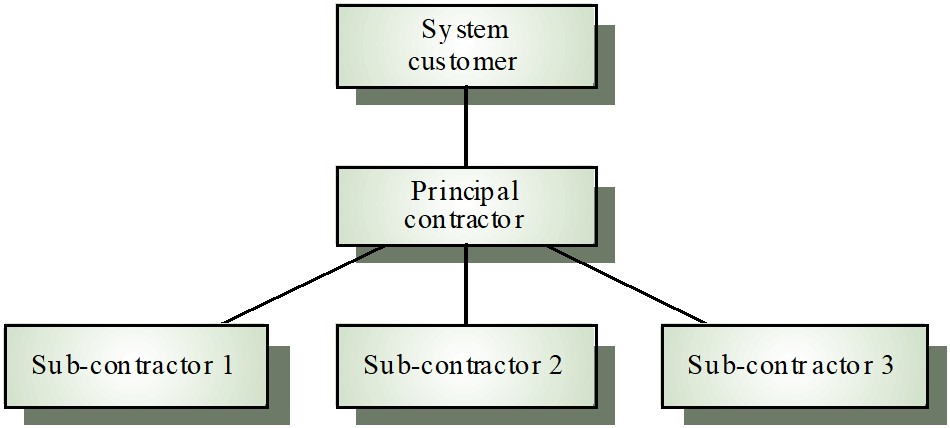
\includegraphics[width=\textwidth]{Contractor-subcontractor.jpg}
\end{itemize}